\chapter{Equilibrio dei fluidi}

I \textbf{fluidi} sono i liquidi e i gas: sostanze che non hanno forma propria e prendono la forma del recipiente che le contiene. A differenza di un corpo solido, un fluido non può ``spingere di taglio'': le forze che scambia con le pareti del recipiente e con i corpi immersi sono sempre \emph{perpendicolari} alle superfici di contatto. Per questo, quando si studia l'equilibrio dei fluidi, la grandezza giusta da usare non è la forza ma la \textbf{pressione}.

\section{La pressione}

Immaginiamo di appoggiare su un tavolo un mattone, prima di piatto e poi di punta. Il peso del mattone è sempre lo stesso, ma nei due casi quel peso si ``spalma'' su un'area di appoggio molto diversa: appoggiando il mattone di punta, la stessa forza agisce su una superficie molto più piccola e il tavolo viene ``premuto'' molto di più in quel punto. La grandezza che misura quanto una forza è concentrata su una superficie è la pressione.

\begin{definizione}
La \textbf{pressione} $p$ è il rapporto fra il modulo della forza $F$ che agisce perpendicolarmente a una superficie e l'area $A$ di quella superficie:
\[ \colorboxed{ocre}{ p = \frac{F}{A}. } \]
\end{definizione}

La pressione è una grandezza \emph{scalare}: non ha una direzione. Nel Sistema Internazionale si misura in \textbf{pascal} (simbolo \si{\pascal}):
\[ \SI{1}{\pascal} = \SI{1}{\newton\per\metre\squared}. \]
Un pascal è una pressione piccolissima (è il peso di circa un etto di pane distribuito su un metro quadrato), quindi nella pratica si usano spesso i suoi multipli: l'ettopascal ($\SI{1}{\hecto\pascal}=\SI{100}{\pascal}$), il chilopascal ($\SI{1}{\kilo\pascal}=\SI{1000}{\pascal}$) e il bar ($\SI{1}{\bar}=\SI{100000}{\pascal}$).

Dalla formula si legge subito che, a parità di forza:
\begin{itemize}
    \item più piccola è l'area di contatto, più grande è la pressione;
    \item più grande è l'area di contatto, più piccola è la pressione.
\end{itemize}
È il motivo per cui un coltello affilato (lama sottile, area piccolissima) taglia, mentre lo stesso coltello con il dorso non fa nulla; ed è il motivo per cui con le racchette da neve non si sprofonda: il peso è lo stesso, ma distribuito su un'area molto maggiore.

\begin{figure}[!htbp]
    \centering
    \begin{tikzpicture}[>=stealth,scale=1]
        % --- caso A: mattone di piatto ---
        \begin{scope}
            \draw[thick] (-0.2,0) -- (3.6,0);
            \fill[pattern=north east lines] (-0.2,-0.25) rectangle (3.6,0);
            \draw[thick,fill=brown!25] (0.4,0) rectangle (3.0,0.9);
            \draw[->,ocre,very thick] (1.7,2.0) -- (1.7,0.95);
            \node[ocre,above] at (1.7,2.0) {$\vec F$};
            \draw[|<->|] (0.4,-0.45) -- (3.0,-0.45);
            \node[below] at (1.7,-0.5) {\footnotesize area $A$ grande};
            \node[below] at (1.7,-1.15) {pressione piccola};
        \end{scope}
        % --- caso B: mattone di punta ---
        \begin{scope}[xshift=6cm]
            \draw[thick] (-0.2,0) -- (2.6,0);
            \fill[pattern=north east lines] (-0.2,-0.25) rectangle (2.6,0);
            \draw[thick,fill=brown!25] (0.85,0) rectangle (1.55,2.6);
            \draw[->,ocre,very thick] (1.2,3.7) -- (1.2,2.65);
            \node[ocre,above] at (1.2,3.7) {$\vec F$};
            \draw[|<->|] (0.85,-0.45) -- (1.55,-0.45);
            \node[below] at (1.2,-0.5) {\footnotesize area $A$ piccola};
            \node[below] at (1.2,-1.15) {pressione grande};
        \end{scope}
    \end{tikzpicture}
    \caption{Lo stesso mattone, con lo stesso peso $\vec F$, appoggiato di piatto e di punta: l'area di contatto $A$ cambia molto, quindi cambia la pressione $p=F/A$ sul piano.}
    \label{fig:pressione-mattone}
\end{figure}

\begin{testexample}[\thetcbcounter \, Pressione di un mattone]
Un mattone pesa $\SI{25}{\newton}$. La faccia più grande misura $\SI{25}{\centi\metre}\times\SI{12}{\centi\metre}$, quella più piccola $\SI{12}{\centi\metre}\times\SI{6}{\centi\metre}$. Calcoliamo la pressione che il mattone esercita sul piano nei due casi.

Le aree, in metri quadrati, valgono
\[ A_1 = 0{,}25\cdot 0{,}12 = \SI{0,030}{\metre\squared}, \qquad
   A_2 = 0{,}12\cdot 0{,}06 = \SI{0,0072}{\metre\squared}. \]
Le pressioni sono quindi
\[ p_1 = \frac{\SI{25}{\newton}}{\SI{0,030}{\metre\squared}} \approx \SI{830}{\pascal}, \qquad
   p_2 = \frac{\SI{25}{\newton}}{\SI{0,0072}{\metre\squared}} \approx \SI{3500}{\pascal}. \]
Appoggiando il mattone di punta la pressione è più di quattro volte maggiore, pur restando invariato il peso.
\end{testexample}

\begin{esercizio}
Una cassa pesa $\SI{600}{\newton}$ e appoggia a terra con una base di $\SI{0,50}{\metre}\times\SI{0,40}{\metre}$. Calcola la pressione esercitata sul pavimento.\\
\risp{$p = \SI{3000}{\pascal}$}
\end{esercizio}

\begin{esercizio}
Un chiodo viene premuto contro una tavola con una forza di $\SI{40}{\newton}$; la punta ha un'area di circa $\SI{0,02}{\milli\metre\squared}$. Che pressione agisce sulla punta? (Esprimi il risultato in \si{\mega\pascal}.)\\
\risp{$p = \SI{2000}{\mega\pascal}$}
\end{esercizio}


\section{La pressione nei liquidi: legge di Stevino}

Un liquido ha un peso, e quel peso preme su tutto ciò che gli sta sotto. Perciò, \textbf{dentro un liquido la pressione non è la stessa dappertutto: cresce con la profondità}. È un fatto che tutti abbiamo sperimentato tuffandoci in piscina: a un paio di metri sotto il pelo dell'acqua si sente la pressione ``spingere'' sui timpani.

Per trovare quanto vale, immaginiamo di isolare, dentro il liquido, una colonna verticale di sezione $A$ che va dalla superficie libera fino a una profondità $h$ (figura~\ref{fig:stevino}). Su quella colonna grava il suo stesso peso:
\[ F = m\,g = \rho\,V\,g = \rho\,(A\,h)\,g, \]
dove $\rho$ è la densità del liquido. Questo peso preme sul fondo della colonna, cioè sul liquido che sta alla profondità $h$, su un'area $A$. La pressione a quella profondità è quindi
\[ p = \frac{F}{A} = \frac{\rho\,A\,h\,g}{A} = \rho\,g\,h. \]

\begin{definizione}
\textbf{Legge di Stevino.} In un liquido di densità $\rho$ in equilibrio, la pressione dovuta al peso del liquido (\emph{pressione idrostatica}) alla profondità $h$ sotto la superficie libera vale
\[ \colorboxed{ocre}{ p = \rho\,g\,h. } \]
\end{definizione}

Guardando la formula si notano tre cose importanti:
\begin{itemize}
    \item la pressione dipende \emph{solo} dalla profondità $h$ e dalla densità $\rho$: \textbf{non} dalla forma del recipiente né dalla quantità totale di liquido. Sul fondo di un sottile tubo alto un metro e sul fondo di un lago profondo un metro (stesso liquido) la pressione è la stessa;
    \item a parità di profondità, un liquido più denso dà una pressione maggiore;
    \item in un punto del liquido la pressione agisce \textbf{ugualmente in tutte le direzioni} (verso il basso, verso l'alto e lateralmente): se così non fosse, il liquido si metterebbe in moto e non sarebbe in equilibrio. Contro una parete, la spinta del liquido è sempre perpendicolare alla parete e cresce scendendo.
\end{itemize}

\begin{figure}[!htbp]
    \centering
    \begin{tikzpicture}[>=stealth,scale=1]
        % liquido
        \fill[blue!10] (0,0) rectangle (5,3.6);
        % recipiente (aperto in alto)
        \draw[thick] (0,4.1) -- (0,0) -- (5,0) -- (5,4.1);
        % superficie libera
        \draw[blue!45!black,thick] (0,3.6) -- (5,3.6);
        \node[blue!45!black,anchor=south west] at (0.1,3.62) {\footnotesize superficie libera};
        % colonna di liquido sovrastante P
        \fill[blue!22] (1.75,1.35) rectangle (2.45,3.6);
        \draw[dashed,gray!65] (1.75,1.35) -- (1.75,3.6)  (2.45,1.35) -- (2.45,3.6);
        \node[gray!55] at (2.1,2.6) {\footnotesize $A$};
        % quota h
        \draw[<->] (0.85,3.6) -- (0.85,1.35) node[midway,fill=blue!10,inner sep=1.5pt] {$h$};
        % punto P e frecce (la pressione agisce ugualmente in ogni direzione)
        \foreach \a in {0,45,...,315}{
            \draw[->,ocre,semithick] (2.1,1.35) -- ++(\a:0.62);}
        \fill (2.1,1.35) circle (1.6pt);
        \node[below left=1pt] at (2.1,1.35) {$P$};
    \end{tikzpicture}
    \caption{La pressione idrostatica nel punto $P$, a profondità $h$, è dovuta al peso della colonna di liquido sovrastante e vale $\rho g h$; in $P$ agisce con lo stesso valore in tutte le direzioni.}
    \label{fig:stevino}
\end{figure}

\subsection{Pressione assoluta e pressione relativa}
Sulla superficie libera del liquido, di solito, non c'è il vuoto ma l'aria, che a sua volta preme con la \emph{pressione atmosferica} $p_0$ (circa \SI{1e5}{\pascal} al livello del mare, ne riparleremo più avanti). Questa pressione si trasmette a tutto il liquido, quindi la pressione \textbf{totale} (o \emph{assoluta}) alla profondità $h$ è
\[ p = p_0 + \rho\,g\,h. \]
Spesso però interessa solo di quanto la pressione supera quella atmosferica -- per esempio è questo che ``sentono'' i timpani, o che misura un manometro: si parla allora di \textbf{pressione relativa}, pari alla sola parte $\rho g h$.

\begin{testexample}[\thetcbcounter \, La pressione a \SI{10}{\metre} sott'acqua]
Calcoliamo la pressione (relativa) dell'acqua ($\rho = \SI{1000}{\kilo\gram\per\metre\cubed}$) alla profondità di \SI{10}{\metre}:
\[ p = \rho\,g\,h = 1000 \cdot 9{,}81 \cdot 10 \approx \SI{98100}{\pascal} \approx \SI{0,98}{\bar}. \]
È quasi esattamente una pressione atmosferica. Vale la regola pratica: \textbf{ogni \SI{10}{\metre} di acqua in più, la pressione aumenta di circa \SI{1}{atm}}. A \SI{10}{\metre} di profondità un sub sopporta quindi una pressione assoluta di circa \SI{2}{atm}, a \SI{20}{\metre} circa \SI{3}{atm}, e così via.
\end{testexample}

\begin{testexample}[\thetcbcounter \, Forza sul timpano di un sub]
Un sub scende in un lago fino a \SI{18}{\metre} di profondità. Il timpano ha un'area di circa \SI{55}{\milli\metre\squared}. Che forza esercita l'acqua sul timpano?

Non c'è una formula unica: bisogna prima trovare la pressione e poi la forza. La pressione relativa alla profondità $h$ è
\[ p = \rho\,g\,h = 1000 \cdot 9{,}81 \cdot 18 \approx \SI{1,77e5}{\pascal}. \]
L'area, in metri quadrati, è $A = \SI{55}{\milli\metre\squared} = \SI{55e-6}{\metre\squared}$. La forza è allora
\[ F = p\,A \approx \SI{1,77e5}{\pascal} \cdot \SI{55e-6}{\metre\squared} \approx \SI{9,7}{\newton}. \]
Quasi un chilogrammo-peso spinge sul timpano da un lato solo: per questo, scendendo, occorre ``compensare'' mandando aria nell'orecchio medio.
\end{testexample}

\begin{testexample}[\thetcbcounter \, Un pilastro e una persona]
Confrontiamo la pressione che un pilastro di cemento ($\rho = \SI{2400}{\kilo\gram\per\metre\cubed}$) a base quadrata di lato \SI{30}{\centi\metre} e alto \SI{4,0}{\metre} esercita sul suolo, con quella di una persona di \SI{70}{\kilo\gram} in piedi su una sola scarpa (area d'appoggio \SI{180}{\centi\metre\squared}).

\emph{Pilastro.} Volume $V = 0{,}30^2 \cdot 4{,}0 = \SI{0,36}{\metre\cubed}$; massa $m = \rho V = 2400 \cdot 0{,}36 = \SI{864}{\kilo\gram}$; peso $P = mg \approx \SI{8480}{\newton}$. La base ha area $A = 0{,}09\ \si{\metre\squared}$, quindi
\[ p_\text{pil} = \frac{P}{A} \approx \frac{8480}{0{,}09} \approx \SI{94000}{\pascal}. \]
\emph{Persona.} $P = 70 \cdot 9{,}81 \approx \SI{687}{\newton}$, $A = \SI{180}{\centi\metre\squared} = \SI{0,018}{\metre\squared}$:
\[ p_\text{pers} = \frac{687}{0{,}018} \approx \SI{38000}{\pascal}. \]
Il pilastro preme sul suolo con una pressione circa $2{,}5$ volte quella della persona.
\end{testexample}

\begin{esercizio}
Nell'acqua di mare ($\rho = \SI{1030}{\kilo\gram\per\metre\cubed}$), a quale profondità la pressione relativa raggiunge \SI{2,5}{\bar}?\\
\risp{$h \approx \SI{24,7}{\metre}$}
\end{esercizio}

\begin{esercizio}
Una vasca di raccolta contiene acqua fino a \SI{1,8}{\metre} di altezza. Su una parete verticale è ricavata una paratoia (uno sportello) rettangolare larga \SI{60}{\centi\metre} e alta \SI{40}{\centi\metre}, il cui bordo inferiore tocca il fondo della vasca. Stima la forza totale con cui l'acqua preme sulla paratoia. \\
\textit{Suggerimento: la pressione non è uniforme; usa il suo valore alla profondità del centro della paratoia.}\\
\risp{$F \approx \SI{3,8e3}{\newton}$}
\end{esercizio}

\begin{esercizio}
Una colonna di \SI{15}{\centi\metre} di mercurio ($\rho = \SI{13600}{\kilo\gram\per\metre\cubed}$) esercita, sul fondo, la stessa pressione di una colonna d'acqua alta quanto? \\
\risp{$h \approx \SI{2,0}{\metre}$}
\end{esercizio}

\begin{esercizio}
Un serbatoio cilindrico vuoto ha massa \SI{40}{\kilo\gram}, diametro \SI{1,2}{\metre} e poggia su 3 piedini, ciascuno con base d'appoggio di \SI{15}{\centi\metre\squared}. Viene riempito di gasolio ($\rho = \SI{840}{\kilo\gram\per\metre\cubed}$) fino all'altezza di \SI{1,5}{\metre}. Calcola la pressione che ciascun piedino esercita sul pavimento.\\
\risp{$p \approx \SI{3,2}{\mega\pascal}$}
\end{esercizio}

\begin{esercizio}
Due recipienti, uno cilindrico stretto e uno largo e svasato, contengono acqua fino alla stessa altezza di \SI{20}{\centi\metre}. In quale dei due la pressione sul fondo è maggiore? Motiva la risposta.\\
\risp{è uguale: la pressione idrostatica dipende solo dall'altezza del liquido, non dalla forma né dal volume}
\end{esercizio}


\section{Il principio di Pascal}

Nella legge di Stevino abbiamo considerato la pressione dovuta al \emph{peso} del liquido. Ma se sul liquido, chiuso in un recipiente, agisce anche una pressione dall'esterno -- per esempio la mano che spinge sul tappo di una siringa piena d'acqua -- che fine fa quella pressione?

L'esperienza dice che si trasmette dappertutto: se buchiamo la siringa in un punto qualsiasi, l'acqua schizza fuori con la stessa forza. Lo enunciò a metà del Seicento il matematico e fisico francese Blaise Pascal.

\begin{definizione}
\textbf{Principio di Pascal.} Una pressione esercitata sulla superficie di un liquido racchiuso si trasmette \textbf{inalterata} a ogni punto del liquido e a tutte le pareti del recipiente, qualunque sia la loro orientazione.
\end{definizione}

La pressione totale in un punto del liquido è quindi la somma di quella esterna e di quella idrostatica di Stevino, come già visto per la pressione atmosferica: $p = p_\text{esterna} + \rho g h$.

\subsection{Il torchio idraulico}
La conseguenza più utile del principio di Pascal è una macchina capace di \textbf{moltiplicare le forze}: il \textbf{torchio idraulico} (o pressa idraulica). Due cilindri di sezione diversa, $A_1$ piccola e $A_2$ grande, sono collegati sul fondo e riempiti di un liquido; ciascuno è chiuso da un pistone (figura~\ref{fig:torchio}).

Se sul pistone piccolo premiamo con una forza $F_1$, nel liquido nasce una pressione
\[ p = \frac{F_1}{A_1}, \]
che per il principio di Pascal si ritrova identica sotto il pistone grande. Là questa pressione agisce sull'area $A_2$ e produce una forza
\[ \colorboxed{ocre}{ F_2 = p\,A_2 = F_1\,\frac{A_2}{A_1}. } \]
Poiché $A_2 > A_1$, la forza $F_2$ è \emph{più grande} di $F_1$, tante volte quanto è il rapporto fra le aree. Con un cilindro grande $50$ volte quello piccolo, una spinta di \SI{200}{\newton} sul pistone piccolo diventa una spinta di \SI{10000}{\newton} sul pistone grande: abbastanza da sollevare un'automobile.

\begin{figure}[!htbp]
    \centering
    \begin{tikzpicture}[>=stealth,scale=1]
        % liquido (canale + due colonne)
        \fill[blue!12] (1.0,0) rectangle (5.6,0.5);
        \fill[blue!12] (1.0,0.5) rectangle (1.8,2.55);
        \fill[blue!12] (3.4,0.5) rectangle (5.6,2.95);
        % pareti del torchio (tubo a U)
        \draw[thick] (1.0,3.2) -- (1.0,0) -- (5.6,0) -- (5.6,3.6);
        \draw[thick] (1.8,3.2) -- (1.8,0.5) -- (3.4,0.5) -- (3.4,3.6);
        % pistone piccolo + stelo
        \fill[gray!35] (1.02,2.55) rectangle (1.78,2.85);
        \draw[thick] (1.02,2.55) rectangle (1.78,2.85);
        \draw[thick] (1.4,2.85) -- (1.4,3.35);
        % pistone grande + carico
        \fill[gray!35] (3.42,2.95) rectangle (5.58,3.25);
        \draw[thick] (3.42,2.95) rectangle (5.58,3.25);
        \draw[thick,fill=gray!45] (4.0,3.25) rectangle (5.0,3.75);
        % forze
        \draw[->,red!70!black,very thick] (1.4,4.15) -- (1.4,3.4);
        \node[red!70!black,above] at (1.4,4.15) {$\vec F_1$};
        \draw[->,ocre,very thick] (4.5,3.75) -- (4.5,3.28);
        \node[ocre,anchor=west] at (5.1,3.9) {$\vec F_2$ (carico)};
        % aree
        \draw[<->] (1.02,2.35) -- (1.78,2.35);
        \node[below,font=\footnotesize] at (1.4,2.33) {$A_1$};
        \draw[<->] (3.42,2.7) -- (5.58,2.7);
        \node[below,font=\footnotesize] at (4.5,2.68) {$A_2$};
    \end{tikzpicture}
    \caption{Torchio idraulico. La pressione prodotta dalla piccola forza $F_1$ sull'area $A_1$ si trasmette inalterata sotto il pistone grande, dove sull'area $A_2$ dà una forza $F_2 = F_1\,A_2/A_1$, molto maggiore.}
    \label{fig:torchio}
\end{figure}

\begin{remark}
Il torchio idraulico non ``crea'' energia. Quando il pistone piccolo scende di un tratto $d_1$, sposta un volume di liquido $A_1 d_1$ che fa salire il pistone grande di un tratto $d_2$ molto minore, tale che $A_1 d_1 = A_2 d_2$. Si ha allora $F_1 d_1 = F_2 d_2$: si guadagna in forza esattamente quanto si perde in spostamento, come per le leve. Per sollevare un carico di parecchio, il pistone piccolo va pompato molte volte.
\end{remark}

\begin{testexample}[\thetcbcounter \, Un cric idraulico]
Il cric idraulico di un'officina ha il pistone di spinta di sezione $A_1 = \SI{2,0}{\centi\metre\squared}$ e quello di sollevamento di sezione $A_2 = \SI{50}{\centi\metre\squared}$. Vogliamo sollevare un'auto che grava sul cric con \SI{6000}{\newton}.

\emph{Forza da applicare.} Serve che $F_2 = \SI{6000}{\newton}$, quindi
\[ F_1 = F_2\,\frac{A_1}{A_2} = 6000 \cdot \frac{2{,}0}{50} = \SI{240}{\newton}. \]
\emph{Quante pompate.} Ogni corsa del pistone piccolo è lunga $d_1 = \SI{3,0}{\centi\metre}$. Il volume spostato a ogni corsa è $A_1 d_1$; per far salire l'auto di $d_2 = \SI{12}{\centi\metre}$ serve un volume totale $A_2 d_2$. Il numero di pompate è
\[ n = \frac{A_2\,d_2}{A_1\,d_1} = \frac{50 \cdot 12}{2{,}0 \cdot 3{,}0} = 100. \]
\end{testexample}

\begin{esercizio}
In un torchio idraulico i pistoni hanno diametri di \SI{4,0}{\centi\metre} e \SI{32}{\centi\metre}. Che forza va applicata al pistone piccolo per equilibrare un carico di \SI{9,6}{\kilo\newton} su quello grande?\\
\risp{$F_1 = \SI{150}{\newton}$}
\end{esercizio}

\begin{esercizio}
Un sollevatore idraulico solleva un carico di \SI{12}{\kilo\newton} spingendo sul pistone piccolo (sezione \SI{5,0}{\centi\metre\squared}) con una forza di \SI{80}{\newton}. Qual è la sezione del pistone grande? Se il pistone piccolo compie corse di \SI{40}{\centi\metre}, quante corse servono per alzare il carico di \SI{25}{\centi\metre}?\\
\risp{$A_2 = \SI{750}{\centi\metre\squared}$; \; $n \approx 94$ corse}
\end{esercizio}

\begin{esercizio}
Spiega perché, nell'impianto frenante di un'automobile, una pressione modesta del piede sul pedale produce sulle pastiglie una forza molto grande.\\
\risp{la pressione si trasmette inalterata (Pascal) dal cilindretto del pedale ai pistoncini delle pinze, che hanno area totale molto maggiore: $F = p\,A$ cresce con l'area}
\end{esercizio}


\section{I vasi comunicanti}

Se colleghiamo con un tubo due o più recipienti -- i \textbf{vasi comunicanti} -- e versiamo un liquido in uno di essi, il liquido si distribuisce fra tutti e si ferma quando ha raggiunto \textbf{lo stesso livello in ciascuno}, indipendentemente dalla forma e dalla larghezza dei recipienti (figura~\ref{fig:vasi}).

\begin{figure}[!htbp]
    \centering
    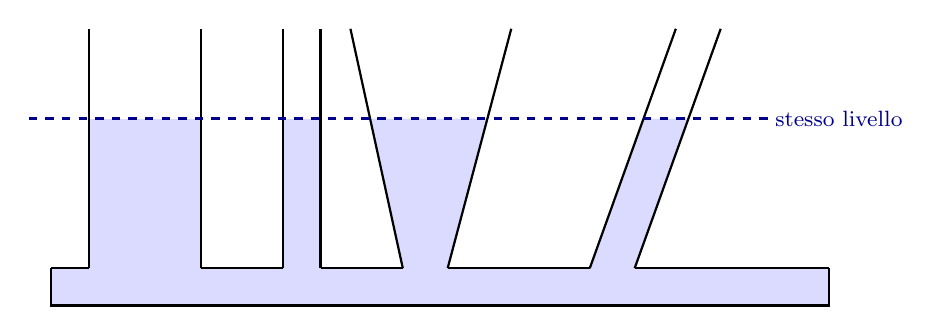
\begin{tikzpicture}[scale=0.95]
        % --- liquido: tubo di base + colonne fino al livello y=2.5 ---
        \fill[blue!14] (0,0) rectangle (10.4,0.5);
        \fill[blue!14] (0.5,0.5) rectangle (2.0,2.5);                  % vaso A
        \fill[blue!14] (3.1,0.5) rectangle (3.6,2.5);                  % vaso B
        \fill[blue!14] (4.7,0.5) -- (5.3,0.5) -- (5.83,2.5) -- (4.26,2.5) -- cycle; % vaso C
        \fill[blue!14] (7.2,0.5) -- (7.8,0.5) -- (8.52,2.5) -- (7.92,2.5) -- cycle; % vaso D
        % --- pareti dei vasi ---
        \draw[thick] (0.5,3.7) -- (0.5,0.5)  (2.0,0.5) -- (2.0,3.7);
        \draw[thick] (3.1,3.7) -- (3.1,0.5)  (3.6,0.5) -- (3.6,3.7);
        \draw[thick] (4.0,3.7) -- (4.7,0.5)  (5.3,0.5) -- (6.15,3.7);
        \draw[thick] (8.35,3.7) -- (7.2,0.5)  (7.8,0.5) -- (8.95,3.7);
        % --- tubo di base (contorno) ---
        \draw[thick] (0,0.5) -- (0,0) -- (10.4,0) -- (10.4,0.5);
        \draw[thick] (0,0.5) -- (0.5,0.5)  (2.0,0.5) -- (3.1,0.5)
                     (3.6,0.5) -- (4.7,0.5)  (5.3,0.5) -- (7.2,0.5)
                     (7.8,0.5) -- (10.4,0.5);
        % --- livello comune ---
        \draw[dashed,blue!55!black,thick] (-0.3,2.5) -- (9.6,2.5);
        \node[blue!55!black,anchor=west,font=\footnotesize] at (9.55,2.5) {stesso livello};
    \end{tikzpicture}
    \caption{Vasi comunicanti: uno stesso liquido raggiunge in tutti i recipienti lo stesso livello, qualunque sia la loro forma.}
    \label{fig:vasi}
\end{figure}

\paragraph{Perché.} Consideriamo il sottile strato di liquido che sta nel tubo di collegamento fra due vasi. Da sinistra il liquido lo preme con la pressione idrostatica $\rho g h_1$ (dove $h_1$ è l'altezza del liquido nel vaso di sinistra sopra il tubo); da destra con $\rho g h_2$. Se il liquido è fermo, quello strato è in equilibrio e le due pressioni sono uguali:
\[ \rho\,g\,h_1 = \rho\,g\,h_2 \qquad\Longrightarrow\qquad \colorboxed{ocre}{ h_1 = h_2. } \]
Il livello dipende solo dalla pressione, e la pressione (legge di Stevino) dipende solo dall'altezza: quindi i livelli si pareggiano.

\subsection{Applicazioni}
\begin{elenco}
    \item \textbf{Indicatore di livello.} A una cisterna chiusa si collega, sul fondo, un tubo verticale trasparente e graduato. Per i vasi comunicanti il liquido nel tubo sale fino allo stesso livello che ha nella cisterna: si legge così dall'esterno quanto liquido c'è dentro.
    \item \textbf{Rete idrica.} L'acqua di un acquedotto arriva ai rubinetti perché parte da un serbatoio posto \emph{più in alto} (una torre piezometrica, o un serbatoio in collina). L'acqua può salire nelle case solo fino al livello di quel serbatoio: ai piani più alti di quella quota il rubinetto non dà acqua senza una pompa.
    \item \textbf{Livella ad acqua.} Due recipienti trasparenti uniti da un tubo flessibile pieno d'acqua: i due peli liberi sono sempre alla stessa quota, e permettono di riportare un livello di riferimento da un punto all'altro di un cantiere, anche dietro un ostacolo.
    \item \textbf{Chiuse dei canali.} Per far superare a una barca un dislivello, si chiude un tratto di canale fra due porte e lo si riempie o svuota finché il livello dell'acqua non pareggia quello a monte o a valle.
\end{elenco}

\subsection{Vasi comunicanti con due liquidi}
Il livello si pareggia solo se il liquido è \emph{uno solo}. Se in un tubo a U mettiamo due liquidi che non si mescolano -- per esempio acqua e olio -- essi si dispongono con l'olio (meno denso) sopra e, nei due rami, a \textbf{altezze diverse} (figura~\ref{fig:utubo}).

All'altezza della superficie di separazione fra i due liquidi, la pressione deve essere la stessa nei due rami. Nel ramo con il liquido~1 (altezza $h_1$ sopra quella superficie) vale $\rho_1 g h_1$; nell'altro $\rho_2 g h_2$. Dall'uguaglianza:
\[ \rho_1\,g\,h_1 = \rho_2\,g\,h_2 \qquad\Longrightarrow\qquad \colorboxed{ocre}{ \rho_1\,h_1 = \rho_2\,h_2. } \]
Le altezze delle due colonne sono \emph{inversamente proporzionali} alle densità: il liquido più denso forma la colonna più bassa. Misurando $h_1$ e $h_2$ si può ricavare la densità di un liquido, note quella dell'altro.

\begin{figure}[!htbp]
    \centering
    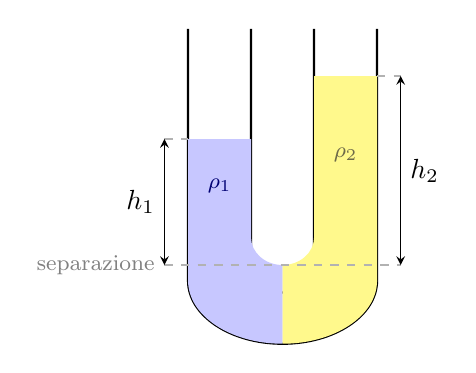
\begin{tikzpicture}[>=stealth,scale=1]
        % tubo a U (pareti)
        \draw[thick] (0,4) -- (0,0.8) arc (180:360:1.2 and 0.8) -- (2.4,4);
        \draw[thick] (0.8,4) -- (0.8,1.0) arc (180:360:0.4 and 0.35) -- (1.6,4);
        % liquido 1 (denso) a sinistra
        \fill[blue!22] (0,0.8) arc (180:270:1.2 and 0.8) -- (1.2,1.0)
            arc (270:180:0.4 and 0.35) -- (0.8,2.6) -- (0,2.6) -- cycle;
        % liquido 2 (leggero) a destra
        \fill[yellow!45] (2.4,0.8) arc (0:-90:1.2 and 0.8) -- (1.2,1.0)
            arc (-90:0:0.4 and 0.35) -- (1.6,3.4) -- (2.4,3.4) -- cycle;
        % superficie di separazione
        \draw[dashed,gray!60] (-0.3,1.0) -- (2.7,1.0);
        \node[gray,anchor=east,font=\footnotesize] at (-0.3,1.0) {separazione};
        % livelli
        \draw[dashed,gray!60] (-0.3,2.6) -- (0,2.6);
        \draw[dashed,gray!60] (2.4,3.4) -- (2.7,3.4);
        \draw[<->] (-0.3,1.0) -- (-0.3,2.6) node[midway,left] {$h_1$};
        \draw[<->] (2.7,1.0) -- (2.7,3.4) node[midway,right] {$h_2$};
        \node[font=\footnotesize] at (-0.4,1.8) {};
        \node[blue!45!black,font=\footnotesize] at (0.4,2.0) {$\rho_1$};
        \node[yellow!35!black,font=\footnotesize] at (2.0,2.4) {$\rho_2$};
    \end{tikzpicture}
    \caption{Due liquidi non miscibili in un tubo a U: il più denso ($\rho_1$) forma la colonna più bassa. All'altezza della superficie di separazione le pressioni si equilibrano: $\rho_1 h_1 = \rho_2 h_2$.}
    \label{fig:utubo}
\end{figure}

\begin{testexample}[\thetcbcounter \, Densità di un olio con il tubo a U]
In un tubo a U c'è dell'acqua ($\rho_\text{acqua} = \SI{1000}{\kilo\gram\per\metre\cubed}$). Versando dell'olio in un ramo, questo forma una colonna alta \SI{12,0}{\centi\metre}; nell'altro ramo l'acqua, rispetto alla superficie di separazione, è salita di \SI{10,4}{\centi\metre}. Qual è la densità dell'olio?

All'altezza della separazione le pressioni sono uguali: $\rho_\text{olio}\,h_\text{olio} = \rho_\text{acqua}\,h_\text{acqua}$, quindi
\[ \rho_\text{olio} = \rho_\text{acqua}\,\frac{h_\text{acqua}}{h_\text{olio}} = 1000 \cdot \frac{10{,}4}{12{,}0} \approx \SI{870}{\kilo\gram\per\metre\cubed}. \]
\end{testexample}

\begin{esercizio}
Il serbatoio pensile di un paese ha il pelo libero dell'acqua a \SI{34}{\metre} sopra la strada. Un palazzo alto \SI{30}{\metre} riceve l'acqua a tutti i piani? E se costruissero un attico che porta l'altezza a \SI{36}{\metre}?\\
\risp{sì fino a \SI{34}{\metre}; l'attico a \SI{36}{\metre} resterebbe senz'acqua (serve una pompa o un'autoclave)}
\end{esercizio}

\begin{esercizio}
In un tubo a U si versa mercurio ($\rho = \SI{13600}{\kilo\gram\per\metre\cubed}$); poi, in un ramo, si aggiunge acqua fino a formare una colonna di \SI{20}{\centi\metre} sopra la superficie di contatto. Di quanto si alza il mercurio nell'altro ramo rispetto a quella superficie?\\
\risp{$h_\text{Hg} \approx \SI{1,5}{\centi\metre}$}
\end{esercizio}

\begin{esercizio}
Due tubi verticali, uno di sezione \SI{1}{\centi\metre\squared} e uno di sezione \SI{20}{\centi\metre\squared}, sono collegati sul fondo e contengono acqua. Si versano \SI{100}{\milli\litre} d'acqua nel tubo sottile. Di quanto sale il livello (uguale nei due)?\\
\risp{$\Delta h \approx \SI{4,8}{\centi\metre}$}
\end{esercizio}

\begin{esercizio}
Perché la superficie libera dell'acqua di un lago tranquillo è orizzontale, mentre quella dell'acqua che scorre in un fiume in pendenza non lo è?\\
\risp{in equilibrio i punti alla stessa quota devono avere la stessa pressione (vasi comunicanti): la superficie libera è orizzontale. L'acqua di un fiume non è in equilibrio, è in moto}
\end{esercizio}


\section{La pressione atmosferica}\label{sec:atm}

Anche l'aria è un fluido e ha un peso. La Terra è avvolta da uno strato di aria -- l'\textbf{atmosfera} -- alto oltre un centinaio di chilometri; il peso di tutta quest'aria preme su ogni corpo che si trova sulla superficie terrestre. Questa pressione si chiama \textbf{pressione atmosferica}, $p_0$.

Non la avvertiamo perché agisce ugualmente da tutte le parti, e perché i fluidi del nostro corpo spingono verso l'esterno con la stessa pressione. Ma c'è: se togliamo l'aria da un recipiente a pareti sottili (una lattina, una bottiglia di plastica), la pressione esterna lo schiaccia.

\subsection{L'esperimento di Torricelli}
Nel 1643 Evangelista Torricelli, allievo di Galileo, misurò per la prima volta la pressione atmosferica. Prese un tubo di vetro lungo circa un metro, chiuso a un'estremità, lo riempì completamente di mercurio, lo tappò con un dito e lo capovolse immergendo l'estremità aperta in una vaschetta piena di mercurio (figura~\ref{fig:torricelli}). Tolto il dito, il mercurio nel tubo scese, ma non del tutto: si fermò formando una colonna alta circa \textbf{\SI{76}{\centi\metre}} sopra il livello della vaschetta. Sopra il mercurio, nel tubo, restò uno spazio \emph{vuoto} (il ``vuoto di Torricelli'').

\begin{figure}[!htbp]
    \centering
    \begin{tikzpicture}[>=stealth,scale=1]
        % vaschetta di mercurio
        % vaschetta di mercurio
        \fill[gray!45] (0,0) rectangle (5.4,1.0);
        \draw[thick] (0,1.5) -- (0,0) -- (5.4,0) -- (5.4,1.5);
        \node[anchor=east,font=\footnotesize] at (0,0.5) {mercurio};
        % tubo (chiuso in alto, immerso in basso)
        \draw[thick] (2.5,0.35) -- (2.5,6.0) -- (3.0,6.0) -- (3.0,0.35);
        % mercurio nel tubo, fino a 76 (scala: 1 unita' = ~16 cm -> colonna 4.75)
        \fill[gray!45] (2.5,0.35) rectangle (3.0,5.1);
        % vuoto sopra la colonna
        \node[anchor=west,font=\footnotesize] at (3.25,5.6) {vuoto};
        \draw[->] (3.2,5.6) -- (2.9,5.6);
        % quota della colonna, misurata dal pelo libero della vaschetta
        \draw[dashed,gray!55] (1.4,1.0) -- (2.5,1.0);
        \draw[dashed,gray!55] (3.0,5.1) -- (3.9,5.1);
        \draw[<->] (1.7,1.0) -- (1.7,5.1)
            node[midway,fill=white,inner sep=1.5pt,font=\footnotesize] {$\approx \SI{76}{\centi\metre}$};
        % pressione atmosferica sul pelo libero
        \foreach \x in {0.5,1.1,1.7,3.8,4.4,5.0}{
            \draw[->,ocre,thick] (\x,2.0) -- (\x,1.05);}
        \node[ocre,anchor=west,font=\footnotesize] at (3.6,2.3) {$p_0$ (atmosfera)};
    \end{tikzpicture}
    \caption{L'esperimento di Torricelli. La pressione atmosferica $p_0$ preme sulla superficie del mercurio nella vaschetta e regge, nel tubo, una colonna di mercurio alta circa \SI{76}{\centi\metre}. Sopra la colonna c'è il vuoto.}
    \label{fig:torricelli}
\end{figure}

\paragraph{Perché.} Consideriamo il mercurio all'imboccatura del tubo, al livello della superficie libera nella vaschetta. Da fuori, la pressione atmosferica preme sulla vaschetta e si trasmette fin lì (principio di Pascal). Da dentro il tubo preme solo il peso della colonna di mercurio, cioè la pressione di Stevino $\rho_\text{Hg}\,g\,h$ (sopra c'è il vuoto, che non pesa). All'equilibrio le due pressioni sono uguali:
\[ \colorboxed{ocre}{ p_0 = \rho_\text{Hg}\,g\,h. } \]

Con $\rho_\text{Hg} = \SI{13600}{\kilo\gram\per\metre\cubed}$ e $h = \SI{0,76}{\metre}$:
\[ p_0 = 13600 \cdot 9{,}81 \cdot 0{,}76 \approx \SI{1,01e5}{\pascal}. \]

\subsection{Le unità di pressione atmosferica}
Il valore trovato da Torricelli serve da riferimento e dà origine a diverse unità pratiche:
\begin{itemize}
    \item l'\textbf{atmosfera}: $\SI{1}{atm} = \SI{101325}{\pascal}$ (per definizione);
    \item il \textbf{millimetro di mercurio} (o \emph{torr}): la pressione di \SI{1}{\milli\metre} di mercurio, circa \SI{133}{\pascal}. Quindi $\SI{1}{atm} = \SI{760}{\mmHg}$. È l'unità usata per la pressione del sangue;
    \item il \textbf{bar} e l'\textbf{ettopascal}: $\SI{1}{\bar} = \SI{1e5}{\pascal}$, $\SI{1}{\hecto\pascal} = \SI{100}{\pascal} = \SI{1}{mbar}$. I bollettini meteo danno la pressione in hPa: circa \SI{1013}{\hecto\pascal} in condizioni normali.
\end{itemize}
Lo strumento che misura la pressione atmosferica si chiama \textbf{barometro} (a mercurio, come quello di Torricelli, oppure metallico -- \emph{aneroide}).

\begin{remark}
Perché Torricelli usò il mercurio e non l'acqua? Perché l'acqua è $13{,}6$ volte meno densa: una ``colonna d'acqua'' capace di reggere la pressione atmosferica sarebbe alta
\[ h = \frac{p_0}{\rho_\text{acqua}\,g} = \frac{\SI{1,01e5}{\pascal}}{1000 \cdot 9{,}81} \approx \SI{10,3}{\metre}, \]
un tubo impraticabile. Questo spiega anche perché una pompa aspirante non riesce a ``tirare su'' l'acqua da un pozzo più profondo di circa \SI{10}{\metre}.
\end{remark}

La pressione atmosferica \textbf{diminuisce con la quota}, perché salendo si lascia sotto di sé una parte sempre maggiore dell'aria: è circa \SI{1013}{\hecto\pascal} al livello del mare, scende a circa \SI{900}{\hecto\pascal} a \SI{1000}{\metre} e a circa \SI{700}{\hecto\pascal} a \SI{3000}{\metre}. Gli altimetri degli aerei e degli orologi da montagna sfruttano proprio questa variazione.

\begin{testexample}[\thetcbcounter \, La forza dell'aria su un banco]
Il piano di un banco misura $\SI{120}{\centi\metre}\times\SI{60}{\centi\metre}$. Con quale forza l'aria preme sulla sua faccia superiore?

L'area è $A = 1{,}20 \cdot 0{,}60 = \SI{0,72}{\metre\squared}$. Con $p_0 \approx \SI{1,0e5}{\pascal}$:
\[ F = p_0\,A \approx 1{,}0\cdot 10^5 \cdot 0{,}72 \approx \SI{72000}{\newton}, \]
il peso di più di sette tonnellate! Non schiaccia il banco solo perché la stessa aria preme con \SI{72000}{\newton} anche \emph{da sotto}, e le due forze si annullano.
\end{testexample}

\begin{esercizio}
Esprimi in pascal e in atmosfere una pressione arteriosa di \SI{120}{\mmHg} ($\SI{1}{\mmHg} \approx \SI{133}{\pascal}$).\\
\risp{$\approx \SI{16000}{\pascal} \approx 0{,}16\ \si{atm}$}
\end{esercizio}

\begin{esercizio}
In cima a una montagna un barometro segna \SI{760}{\hecto\pascal}, mentre a valle segna \SI{1000}{\hecto\pascal}. Stimando la densità media dell'aria in \SI{1,2}{\kilo\gram\per\metre\cubed}, quanto è alta all'incirca la montagna rispetto al fondovalle?\\
\risp{$\approx \SI{2000}{\metre}$}
\end{esercizio}

\begin{esercizio}
Un tubo lungo \SI{1,0}{\metre}, chiuso a un'estremità, viene riempito d'acqua e capovolto in una bacinella d'acqua, come nell'esperimento di Torricelli. Che cosa si osserva?\\
\risp{il tubo resta pieno: la pressione atmosferica regge una colonna d'acqua fino a $\sim\SI{10}{\metre}$, quindi $\SI{1}{\metre}$ non basta a farla scendere}
\end{esercizio}

\begin{esercizio}
Due emisferi metallici vengono accostati e si fa il vuoto al loro interno. Il loro cerchio di contatto ha un diametro di \SI{30}{\centi\metre}. Stima la forza minima necessaria per staccarli (emisferi di Magdeburgo).\\
\risp{$F \approx p_0 \cdot \pi r^2 \approx \SI{7,1e3}{\newton}$}
\end{esercizio}


\section{Il principio di Archimede}

Un corpo immerso in un liquido sembra ``pesare di meno'': lo sappiamo tutti dall'esperienza di sollevare un sasso sott'acqua. Il motivo è che il liquido spinge il corpo verso l'\emph{alto} con una forza detta \textbf{spinta di Archimede} (o spinta idrostatica).

La spinta nasce dalla legge di Stevino. La pressione del liquido sulla faccia \emph{inferiore} del corpo, che è più in profondità, è maggiore di quella sulla faccia \emph{superiore}: le forze di pressione non si bilanciano e ne resta una risultante diretta verso l'alto.

\subsection{Quanto vale la spinta}
Immaginiamo di togliere il corpo e di rimpiazzarlo con altro liquido, che occupi esattamente lo stesso spazio. Quella ``bolla'' di liquido è in equilibrio: il suo peso (verso il basso) è bilanciato esattamente dalla spinta che il liquido circostante esercita su di essa (verso l'alto). Ma il liquido circostante non sa che cosa c'è dentro quello spazio: eserciterebbe la stessa spinta su qualunque corpo lo occupasse. Quindi:

\begin{definizione}
\textbf{Principio di Archimede.} Un corpo immerso in un fluido riceve una spinta verticale verso l'alto uguale al \textbf{peso del fluido spostato}:
\[ \colorboxed{ocre}{ S = \rho_\text{fluido}\; V_\text{imm}\; g, } \]
dove $\rho_\text{fluido}$ è la densità del fluido e $V_\text{imm}$ è il volume della parte di corpo immersa (il volume di fluido spostato).
\end{definizione}

Su un corpo immerso agiscono quindi \textbf{due} forze verticali: il peso $\vec P = \rho_\text{c}\,V_\text{c}\,g$ verso il basso (dove $\rho_\text{c}$ e $V_\text{c}$ sono densità e volume del corpo) e la spinta $\vec S$ verso l'alto.

\begin{figure}[!htbp]
    \centering
    \begin{tikzpicture}[>=stealth,scale=1]
        % liquido
        \fill[blue!12] (0,0) rectangle (5,3.4);
        \draw[thick] (0,3.9) -- (0,0) -- (5,0) -- (5,3.9);
        \draw[blue!45!black,thick] (0,3.4) -- (5,3.4);
        % dinamometro (stelo che esce dal liquido)
        \draw[thick] (2.5,5.4) -- (2.5,3.9);
        \draw[thick,decorate,decoration={coil,aspect=0.6,segment length=4pt,amplitude=4pt}] (2.5,5.4) -- (2.5,4.4);
        \draw[thick] (2.5,4.4) -- (2.5,2.3);
        % corpo immerso
        \draw[thick,fill=brown!30] (1.9,1.0) rectangle (3.1,2.3);
        % pressioni sulle facce
        \foreach \x in {2.1,2.5,2.9}{\draw[->,blue!55!black] (\x,2.65) -- (\x,2.35);}
        \foreach \x in {2.0,2.35,2.7,3.05}{\draw[->,blue!55!black,thick] (\x,0.55) -- (\x,0.95);}
        % forze risultanti
        \draw[->,ocre,very thick] (2.5,1.65) -- (2.5,0.2) node[right=1pt,pos=0.85] {$\vec P$};
        \draw[->,blue!60!black,very thick] (3.55,1.65) -- (3.55,3.05) node[right=1pt,pos=0.9] {$\vec S$};
        \draw[dotted] (3.1,1.65) -- (3.55,1.65);
    \end{tikzpicture}
    \caption{Su un corpo immerso il liquido preme di più sulla faccia inferiore (più profonda) che su quella superiore: ne risulta la spinta di Archimede $\vec S$ verso l'alto, che si oppone al peso $\vec P$. Il dinamometro segna il ``peso apparente'' $P-S$.}
    \label{fig:archimede}
\end{figure}

\subsection{Peso apparente e galleggiamento}
Se il corpo è \emph{tutto} immerso, un dinamometro che lo sostiene segna il \textbf{peso apparente}
\[ P_\text{app} = P - S = (\rho_\text{c} - \rho_\text{fluido})\,V_\text{c}\,g. \]
Il segno di questa differenza decide il comportamento di un corpo omogeneo lasciato libero in un liquido:
\begin{elenco}
    \item $\rho_\text{c} > \rho_\text{fluido}$: il peso vince la spinta, il corpo \textbf{affonda};
    \item $\rho_\text{c} < \rho_\text{fluido}$: la spinta vince il peso, il corpo \textbf{sale a galla} e poi galleggia, immerso solo in parte;
    \item $\rho_\text{c} = \rho_\text{fluido}$: peso e spinta si equilibrano, il corpo resta fermo dove si trova (equilibrio indifferente).
\end{elenco}

\begin{figure}[!htbp]
    \centering
    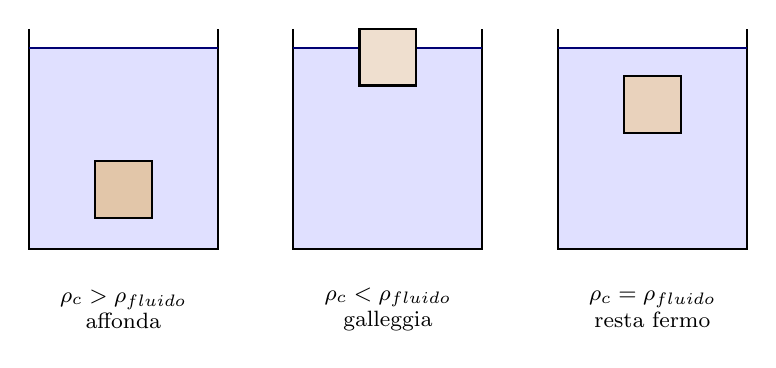
\begin{tikzpicture}[scale=0.8]
        \foreach \i/\lab/\yc/\col in {0/{$\rho_\text{c}>\rho_\text{fluido}$\\ affonda}/0.5/brown!45,
                                     4.2/{$\rho_\text{c}<\rho_\text{fluido}$\\ galleggia}/2.6/brown!25,
                                     8.4/{$\rho_\text{c}=\rho_\text{fluido}$\\ resta fermo}/1.85/brown!35}{
            \begin{scope}[xshift=\i cm]
                \fill[blue!12] (0,0) rectangle (3,3.2);
                \draw[thick] (0,3.5) -- (0,0) -- (3,0) -- (3,3.5);
                \draw[blue!45!black,thick] (0,3.2) -- (3,3.2);
                \draw[thick,fill=\col] (1.05,\yc) rectangle (1.95,\yc+0.9);
                \node[font=\footnotesize,align=center] at (1.5,-0.95) {\lab};
            \end{scope}}
    \end{tikzpicture}
    \caption{Un corpo omogeneo in un liquido: il comportamento dipende dal confronto fra la sua densità e quella del liquido.}
    \label{fig:galleggia}
\end{figure}

Per un corpo che \textbf{galleggia}, all'equilibrio peso e spinta sono uguali, ma ora la spinta usa solo il volume immerso:
\[ \rho_\text{c}\,V_\text{c}\,g = \rho_\text{fluido}\,V_\text{imm}\,g \qquad\Longrightarrow\qquad
   \colorboxed{ocre}{ \frac{V_\text{imm}}{V_\text{c}} = \frac{\rho_\text{c}}{\rho_\text{fluido}}. } \]
La \emph{frazione di volume immersa} è uguale al rapporto fra le densità. Un iceberg ($\rho \approx \SI{920}{\kilo\gram\per\metre\cubed}$) galleggia nell'acqua di mare ($\rho \approx \SI{1025}{\kilo\gram\per\metre\cubed}$) con circa il $90\%$ del volume sott'acqua.

\begin{remark}
Una nave d'acciaio galleggia perché non è un blocco pieno: lo scafo racchiude molta aria, e la \emph{densità media} nave$+$aria è minore di quella dell'acqua. Se lo scafo si squarcia e l'acqua prende il posto dell'aria, la densità media aumenta e la nave affonda. Il sottomarino regola apposta la propria densità media riempiendo o svuotando d'acqua le \emph{casse di zavorra}.
\end{remark}

La spinta di Archimede agisce anche nei gas (\emph{spinta aerostatica}): un pallone gonfio di elio o di aria calda, meno densi dell'aria fredda circostante, riceve una spinta verso l'alto maggiore del proprio peso e si solleva.

\begin{testexample}[\thetcbcounter \, Densità di un oggetto con la bilancia idrostatica]
Un oggetto di metallo pesa \SI{5,40}{\newton} in aria e, appeso a un dinamometro e tenuto immerso in acqua, ne pesa \SI{4,70}{\newton}. Qual è la sua densità?

La differenza fra i due valori è la spinta di Archimede:
\[ S = 5{,}40 - 4{,}70 = \SI{0,70}{\newton}. \]
Poiché $S = \rho_\text{acqua}\,V\,g$, il volume dell'oggetto è
\[ V = \frac{S}{\rho_\text{acqua}\,g} = \frac{0{,}70}{1000 \cdot 9{,}81} \approx \SI{7,1e-5}{\metre\cubed}. \]
La massa dell'oggetto è $m = P/g = 5{,}40/9{,}81 \approx \SI{0,550}{\kilo\gram}$, quindi
\[ \rho_\text{c} = \frac{m}{V} \approx \frac{0{,}550}{\SI{7,1e-5}{}} \approx \SI{7700}{\kilo\gram\per\metre\cubed}. \]
Un valore compatibile con quello del ferro o dell'acciaio.
\end{testexample}

\begin{testexample}[\thetcbcounter \, Una zattera che porta un carico]
Una zattera è fatta di pannelli di polistirolo ($\rho = \SI{25}{\kilo\gram\per\metre\cubed}$) per un volume totale di \SI{0,60}{\metre\cubed}. Quanti chilogrammi di carico può reggere restando appena a galla in acqua dolce?

Al limite del galleggiamento la zattera è tutta immersa e la spinta massima è
\[ S_\text{max} = \rho_\text{acqua}\,V\,g = 1000 \cdot 0{,}60 \cdot 9{,}81 \approx \SI{5890}{\newton}. \]
Questa deve reggere il peso della zattera più quello del carico:
\[ P_\text{zattera} = 25 \cdot 0{,}60 \cdot 9{,}81 \approx \SI{147}{\newton}. \]
Resta per il carico $S_\text{max} - P_\text{zattera} \approx \SI{5740}{\newton}$, cioè una massa di circa
\[ m_\text{carico} = \frac{5740}{9{,}81} \approx \SI{585}{\kilo\gram}. \]
\end{testexample}

\begin{esercizio}
Un cubo di legno di lato \SI{10}{\centi\metre} e densità \SI{700}{\kilo\gram\per\metre\cubed} galleggia in acqua. Quanto sporge dall'acqua?\\
\risp{$\approx \SI{3}{\centi\metre}$}
\end{esercizio}

\begin{esercizio}
Una sfera di alluminio ($\rho = \SI{2700}{\kilo\gram\per\metre\cubed}$) del diametro di \SI{6,0}{\centi\metre} è appesa a un filo e immersa completamente in acqua. Qual è la tensione del filo?\\
\risp{$T = P - S \approx \SI{1,9}{\newton}$}
\end{esercizio}

\begin{esercizio}
Un blocco pesa \SI{12,0}{\newton} in aria e \SI{7,5}{\newton} immerso in acqua. Calcola il suo volume e la sua densità.\\
\risp{$V \approx \SI{4,6e-4}{\metre\cubed}$; \; $\rho_\text{c} \approx \SI{2700}{\kilo\gram\per\metre\cubed}$}
\end{esercizio}

\begin{esercizio}
Una chiatta a fondo piatto ha la base rettangolare di $\SI{8,0}{\metre}\times\SI{3,0}{\metre}$. Caricandola con \SI{6,0}{\tonne}, di quanto si abbassa nell'acqua (dolce)?\\
\risp{$\Delta h = 0{,}25\ \si{\metre}$}
\end{esercizio}

\begin{esercizio}
Un pallone aerostatico ha un volume di \SI{2000}{\metre\cubed} ed è gonfio di elio ($\rho_\text{He} = \SI{0,18}{\kilo\gram\per\metre\cubed}$); l'involucro e la navicella hanno una massa complessiva di \SI{400}{\kilo\gram}. Con quale forza tende a salire, se l'aria ha densità \SI{1,2}{\kilo\gram\per\metre\cubed}? (Trascura il volume di involucro e navicella.)\\
\risp{$S - P \approx \SI{1,6e4}{\newton}$}
\end{esercizio}

\begin{esercizio}
Perché una scialuppa di salvataggio, che è di metallo, galleggia anche quando si riempie parzialmente d'acqua, mentre lo stesso metallo fuso in un blocco affonda?\\
\risp{da vuota, lo scafo racchiude aria e la densità media è minore di quella dell'acqua; il blocco pieno ha la densità (alta) del metallo}
\end{esercizio}
